% Facts: user-supplied paper brief; original paper PDF not available locally.
% Original figure files are preserved. slides/ crops remove captions only.
\documentclass[aspectratio=169,10pt]{beamer}
\usepackage[T1]{fontenc}
\usepackage{lmodern,amsmath,booktabs,tabularx,array,graphicx,tikz}
\usetikzlibrary{arrows.meta,positioning,calc}
\usetheme{Madrid}
\definecolor{Ink}{HTML}{243748}
\definecolor{Muted}{HTML}{667B8B}
\definecolor{Accent}{HTML}{347E74}
\definecolor{SoftBlue}{HTML}{E9F2F9}
\definecolor{Paper}{HTML}{FBFCFE}
\setbeamercolor{background canvas}{bg=Paper}
\setbeamercolor{normal text}{fg=Ink}
\setbeamercolor{structure}{fg=Accent}
\setbeamercolor{frametitle}{fg=Ink,bg=SoftBlue}
\setbeamercolor{block title}{fg=Ink,bg=SoftBlue}
\setbeamercolor{block body}{fg=Ink,bg=white}
\setbeamercolor{footline}{fg=Muted,bg=Paper}
\setbeamerfont{frametitle}{size=\large,series=\bfseries}
\setbeamertemplate{navigation symbols}{}
\setbeamertemplate{headline}{}
\setbeamertemplate{blocks}[rounded][shadow=false]
\setbeamersize{text margin left=.38cm,text margin right=.38cm}
\setbeamertemplate{frametitle}{\nointerlineskip\begin{beamercolorbox}[wd=\paperwidth,sep=.12cm,leftskip=.22cm]{frametitle}\usebeamerfont{frametitle}\strut\insertframetitle\strut\par\end{beamercolorbox}}
\newif\ifbackup
\setbeamertemplate{footline}{\begin{beamercolorbox}[wd=\paperwidth,ht=.30cm,dp=.16cm,rightskip=.50cm]{footline}\hfill\scriptsize\ifbackup Backup PDF \insertframenumber\else Main \insertframenumber/13\fi\end{beamercolorbox}}
\newcommand{\takeaway}[1]{\par\vspace{.12cm}\begin{beamercolorbox}[rounded=true,sep=.12cm,wd=\linewidth]{block title}\small\bfseries #1\end{beamercolorbox}}
\newcommand{\src}[1]{\par\vfill{\fontsize{7}{8}\selectfont\color{Muted}Source: Characterizing High Bandwidth Flash for LLM Serving, #1.}\par}
\newcommand{\fig}[2]{\par{\centering\includegraphics[width=\linewidth,height=#2,keepaspectratio]{CharacterizingHBFforLLMServing/slides/Fig#1.png}\par}}
\newcommand{\head}[1]{\par{\color{Accent}\bfseries #1}\par\smallskip}
\newcommand{\arr}{\,$\rightarrow$\,}
\renewcommand{\arraystretch}{1.15}
\subject{Research meeting, 28 Oct 2026}
\begin{document}
\begin{frame}[t]{Characterizing High Bandwidth Flash for LLM Serving}

\par\vspace{.12cm}
{\Large\color{Accent}When does additional flash capacity\\actually improve LLM serving?\par}
\vspace{.3cm}
Zack Yu et al.\quad arXiv:2609.39131v2, 5 Oct 2026\par
\vspace{.35cm}
\textbf{Yu-Jui Liang}\\[.08cm]
Advisor: Hsiang-Yun Cheng\\[.08cm]
National Taiwan University | Academia Sinica\\[.08cm]
28 Oct 2026
\vspace{.25cm}
\takeaway{HBF helps high-throughput serving mainly by expanding usable device memory, with memory architecture, placement, and scheduling co-designed.}

\src{paper summary; supplied research brief}
\end{frame}

\begin{frame}[t]{Why Does Agentic Serving Need More Device Memory?}

\begin{columns}[T,onlytextwidth]
\begin{column}{.48\textwidth}
\head{Why is HBM capacity a bottleneck?}
\begin{block}{Limited HBM capacity}
Model weights\\[.16cm]
Active request KV\\[.16cm]
Reusable completed-session KV
\end{block}
\small Completed-session KV can be useful again at the next turn.
\end{column}
\begin{column}{.48\textwidth}
\head{One agent session}
\centering Turn 1\par $\downarrow$\par KV generated\par $\downarrow$\par Tool / environment wait\par $\downarrow$\par Turn 2 reuses Turn-1 prefix
\end{column}
\end{columns}
\vspace{.2cm}
\textbf{HBF:} larger package-local capacity.\quad\textbf{Cost:} higher read energy, slow writes, finite endurance.
\takeaway{The opportunity is capacity, but HBF cannot be treated as free extra memory.}

\src{motivation; Table 1}
\end{frame}

\begin{frame}[t]{Two Ways to Add HBF: Shared-Site vs. H$^3$}

\begin{columns}[T,onlytextwidth]
\begin{column}{.59\textwidth}\fig{02}{4.35cm}\end{column}
\begin{column}{.38\textwidth}
\head{Shared-site: fixed 8 sites}
4 HBM + 4 HBF, for example.\\
More HBF sacrifices HBM capacity / bandwidth.
\par\vspace{.12cm}
\head{H$^3$: 8 HBM + 8 HBF}
HBF connects behind HBM. Assumed HBM buffering stages HBF data and hides latency.\\[.12cm]
Full HBM resources, but more stacks and costlier packaging.
\end{column}
\end{columns}
\takeaway{Shared-site trades HBM for HBF; H$^3$ adds HBF without giving up the original HBM capacity.}

\src{Sec. 4.1; Fig. 2}
\end{frame}

\begin{frame}[t]{How Does the HBM--HBF--Host Hierarchy Work?}

\begin{columns}[T,onlytextwidth]
\begin{column}{.34\textwidth}\fig{03}{4.4cm}\end{column}
\begin{column}{.63\textwidth}
\small
\head{HOT: HBM}
Frequent weights, activations, hot index, active / hot KV. New KV and reloaded prefixes enter here.
\vspace{.12cm}\head{HBF $\rightarrow$ host DRAM $\rightarrow$ SSD: COLD}
Request-level LRU demotes older KV. Host holds colder state; SSD is coldest.
\vspace{.12cm}\head{Placement depends on the object}
Activations stay in HBM. Weights stay fixed per configuration. Split MoE: frequent experts in HBM, remaining experts in HBF.
\begin{block}{Index-first under HBM pressure}
Indexer scans context; attention reads Top-K KV. Demote eligible KV before the hotter index.
\end{block}
\end{column}
\end{columns}
\takeaway{The hierarchy treats different objects differently; HBF is not a generic overflow bucket.}

\src{Fig. 3; placement and cache policy}
\end{frame}

\begin{frame}[t]{Why Is Cache-Aware Scheduling Alone Not Enough?}

\begin{columns}[T,onlytextwidth]
\begin{column}{.49\textwidth}
\head{Vanilla cache-aware}\fig{04}{2.35cm}
\small Cache hit first \arr too much active state\\
\arr growing locked KV \arr evict reusable KV\\
\arr future turn loses its cache hit.
\end{column}
\begin{column}{.49\textwidth}
\head{Buffered cache-aware}\fig{05}{2.35cm}
\small $L+A_i\leq bC$,\quad $b=0.9$.\\
$C$: usable KV/index capacity after weights;\\
$L$: locked active state; $A_i$: added locked state.
\end{column}
\end{columns}
\vspace{.14cm}
\small\textbf{10\% is an admission threshold, not a permanently reserved physical partition.} Active contexts can keep growing after admission.\\[.10cm]
Less admission pressure \arr less churn \arr retained prefixes \arr fewer reloads / repeated prefills / HBF writes.
\takeaway{Sacrificing some instantaneous concurrency can improve total throughput by preserving reuse.}

\src{Figs. 4--5; buffered admission policy}
\end{frame}

\begin{frame}[t]{What Exactly Does the Simulator Model?}

\begin{columns}[T,onlytextwidth]
\begin{column}{.55\textwidth}
\head{HBM-only validation against profiled vLLM}
\fig{01}{2.7cm}
\small Llama-3.1-8B on H100; 32--4096 single-turn requests. Mean input 4096; output 128 / 512.\\[.12cm]
\textbf{Throughput MAPE: 9.14\%.}\\
H100/B200 profiling calibrates fitted kernel latency models. Main experiments use B200 compute.
\end{column}
\begin{column}{.42\textwidth}
\centering\small
Request trace\\$\downarrow$\\Scheduler / cache state\\$\downarrow$\\Kernel latency models\\$\downarrow$\\HBM / HBF / DRAM / SSD\\$\downarrow$\\PCIe / NVLink transfer model\\$\downarrow$\\Discrete request-level execution\\$\downarrow$\\Completion time / energy / writes
\end{column}
\end{columns}
\takeaway{Request-level serving simulation with calibrated kernel models. Not a cycle-level GPU simulator.}
\small HBF behavior is extrapolated from assumed specifications.

\src{Fig. 1; simulator methodology}
\end{frame}

\begin{frame}[t]{Experimental Setup: What Workload Stresses HBF?}

\begin{columns}[T,onlytextwidth]
\begin{column}{.46\textwidth}
\head{Session $\neq$ turn}
Session = one agent conversation / trajectory.\\
Turn = one LLM request within it.\\[.15cm]
Session A: Turn 1 \arr gap \arr Turn 2 \arr gap \arr Turn 3
\par\vspace{.12cm}
\head{LMCache workload}
Original: \textbf{24,880 turns / 767 sessions}.\\
25k experiments: 771 sessions.\\
100k experiments: 3,080 sessions.\par
\vspace{.2cm}
\small Qwen3-32B: scheduling / endurance\\
Llama-3.1-405B: dense model\\
GLM-5.2: sparse MoE
\end{column}
\begin{column}{.51\textwidth}
\head{Same 3,080 sessions, longer conversations}
1$\times$: 100k turns, original length pattern\\[.12cm]
{\color{Accent}\rule{1.7cm}{.18cm}}\\[.15cm]
5$\times$: 500k turns, five concatenated copies\\[.12cm]
{\color{Accent}\rule{6.5cm}{.18cm}}\\[.15cm]
Copies continue the preceding context.\\
Mean input: \textbf{22,558 $\rightarrow$ 89,125 tokens}.\\[.2cm]
\textbf{Long-context stress, not merely more independent requests.}
\end{column}
\end{columns}
\takeaway{The 5$\times$ trace tests HBF as per-session KV state grows much larger.}

\src{workload construction; Table 3; bars are schematic}
\end{frame}

\begin{frame}[t]{Q1: Can Scheduling Make HBF KV Writes Sustainable?}

\head{Qwen3-32B: H$^3$ with 8 HBM + 8 HBF}
\begin{tabularx}{\textwidth}{@{}Xrrrr@{}}\toprule
Scheduling & Completion (s)& KV writes (TB)& Device hit& Life (yr)\\\midrule
FCFS &13,552.76&106.79&32.84\%&1.21\\
Cache-aware &10,930.78&21.81&86.87\%&4.77\\
\textbf{Cache-aware + 10\%}&\textbf{10,419.17}&\textbf{6.69}&\textbf{96.46\%}&\textbf{14.82}\\\bottomrule
\end{tabularx}
\vspace{.3cm}
\begin{columns}[T,onlytextwidth]
\begin{column}{.48\textwidth}
\head{Adding the buffer}
HBF writes: 21.81 $\rightarrow$ 6.69 TB\\
{\Large\color{Accent}$-69.33\%$}\\[.12cm]
Completion time: \textbf{$-4.68\%$}
\end{column}
\begin{column}{.48\textwidth}
\head{Estimated lifetime, not measured lifetime}
FCFS $\rightarrow$ buffered: 1.21 $\rightarrow$ 14.82 years.\\[.12cm]
Assumes 100k P/E cycles, uniform wear, and unit write amplification.
\end{column}
\end{columns}
\takeaway{Preserving headroom reduces both churn and write pressure. Endurance depends strongly on serving policy.}

\src{Table 4; simulator lifetime assumptions}
\end{frame}

\begin{frame}[t]{Q2: Does More HBF Capacity Help Dense LLM Serving?}

\head{Llama-3.1-405B: 8 GPUs, TP8, 1$\times$ / 100k turns, 10\% buffer}
\begin{tabularx}{\textwidth}{@{}Xrrr@{}}\toprule
Configuration & Time (s)& Energy (MJ)& TPOT (ms)\\\midrule
HBM-only, HBM weights&39,666&53.60&90.85\\
H$^3$, HBM weights&21,439&40.70&438.61\\
H$^3$, HBF weights&21,423&42.06&438.27\\\bottomrule
\end{tabularx}
\par\vspace{.2cm}
\begin{columns}[T,onlytextwidth]
\begin{column}{.49\textwidth}
\head{Extra capacity helps throughput}
H$^3$ / HBM weights vs. HBM-only:\\
\textbf{45.95\% less completion time};\\
about \textbf{24.1\% less modeled energy}.\\[.13cm]
TPOT: \textbf{90.85 $\rightarrow$ 438.61 ms}.\\
Higher throughput $\neq$ lower request latency.
\end{column}
\begin{column}{.48\textwidth}
\head{Moving hot weights adds little}
21,439 vs. 21,423 s: almost equal.\\
40.70 vs. 42.06 MJ: HBF weights cost \textbf{3.33\% more energy}.\\[.13cm]
Dense weights stay hot; colder KV can reside in HBF.
\end{column}
\end{columns}
\takeaway{Dense Llama benefits mainly from extra KV capacity, not from moving hot weights to HBF.}

\src{Table 5; modeled energy excludes static / background power}
\end{frame}

\begin{frame}[t]{Q3 Setup: DPA Attention $\rightarrow$ TP/EP MoE, Every Layer}

\begin{columns}[T,onlytextwidth]
\begin{column}{.69\textwidth}
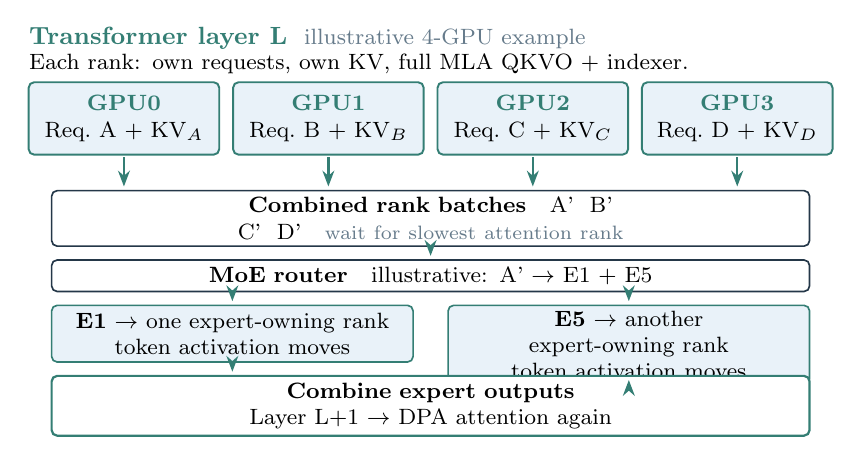
\begin{tikzpicture}[
  font=\footnotesize,
  gpu/.style={draw=Accent, line width=.7pt, rounded corners=2pt, fill=SoftBlue, align=center,
    inner sep=2pt, text width=2.28cm, minimum height=.92cm, outer sep=0pt, font=\footnotesize},
  stage/.style={draw=Ink, line width=.6pt, rounded corners=2pt, fill=white, align=center,
    inner sep=2.5pt, text width=9.45cm, outer sep=0pt, font=\footnotesize},
  expert/.style={draw=Accent, line width=.6pt, rounded corners=2pt, fill=SoftBlue, align=center,
    inner sep=2pt, text width=4.45cm, minimum height=.72cm, outer sep=0pt, font=\footnotesize},
  flowarrow/.style={-{Stealth[length=2mm]}, draw=Accent, line width=.9pt, shorten >=1.5pt, shorten <=1pt}
]
  \node[anchor=north west, inner sep=0pt, font=\small\bfseries, text=Accent] (ltitle) at (0,0) {Transformer layer L};
  \node[anchor=west, inner sep=0pt, font=\footnotesize, text=Muted] at (ltitle.east) {\ \ illustrative 4-GPU example};
  \node[anchor=north west, inner sep=0pt, font=\footnotesize, text width=9.6cm] (dpa) at ([yshift=-1pt]ltitle.south west)
    {Each rank: own requests, own KV, full MLA QKVO + indexer.};
  \node[gpu, anchor=north west] (g0) at ([yshift=-3pt]dpa.south west) {{\color{Accent}\textbf{GPU0}}\par Req.\ A + KV$_A$};
  \node[gpu, anchor=north west] (g1) at ([xshift=5pt]g0.north east) {{\color{Accent}\textbf{GPU1}}\par Req.\ B + KV$_B$};
  \node[gpu, anchor=north west] (g2) at ([xshift=5pt]g1.north east) {{\color{Accent}\textbf{GPU2}}\par Req.\ C + KV$_C$};
  \node[gpu, anchor=north west] (g3) at ([xshift=5pt]g2.north east) {{\color{Accent}\textbf{GPU3}}\par Req.\ D + KV$_D$};
  \coordinate (rowmid) at ($({g0.west})!0.5!({g3.east})$);
  \coordinate (belowrow) at (g0.south -| rowmid);
  \node[stage, anchor=north] (comb) at ([yshift=-13pt]belowrow) {%
    \textbf{Combined rank batches}\quad A' \ B' \ C' \ D'\quad{\scriptsize\color{Muted}wait for slowest attention rank}};
  \draw[flowarrow] (g0.south) -- (g0.south |- comb.north);
  \draw[flowarrow] (g1.south) -- (g1.south |- comb.north);
  \draw[flowarrow] (g2.south) -- (g2.south |- comb.north);
  \draw[flowarrow] (g3.south) -- (g3.south |- comb.north);
  \node[stage, anchor=north] (router) at ([yshift=-5pt]comb.south) {%
    \textbf{MoE router}\quad illustrative: A' $\rightarrow$ E1 + E5};
  \draw[flowarrow] (comb.south) -- (router.north);
  \node[expert, anchor=north west] (e1) at ([yshift=-5pt]router.south west)
    {\textbf{E1} $\rightarrow$ one expert-owning rank\par token activation moves};
  \node[expert, anchor=north east] (e5) at ([yshift=-5pt]router.south east)
    {\textbf{E5} $\rightarrow$ another expert-owning rank\par token activation moves};
  \draw[flowarrow] (e1.north |- router.south) -- (e1.north);
  \draw[flowarrow] (e5.north |- router.south) -- (e5.north);
  \coordinate (nextpos) at (e1.south -| comb.center);
  \node[stage, anchor=north, draw=Accent, line width=.8pt] (next) at ([yshift=-5pt]nextpos) {%
    \textbf{Combine expert outputs}\par Layer L+1 $\rightarrow$ DPA attention again};
  \draw[flowarrow] (e1.south) -- (e1.south |- next.north);
  \draw[flowarrow] (e5.south) -- (e5.south |- next.north);
\end{tikzpicture}
\end{column}
\begin{column}{.29\textwidth}
\footnotesize
{\color{Accent}\bfseries TP / EP}\par
TP: shard tensor computation.\par
EP: route tokens to experts.
\par\vspace{.05cm}
{\color{Accent}\bfseries Weights stay fixed}\par
Non-expert weights fixed per configuration.\par
Split: hot $\rightarrow$ HBM, rest $\rightarrow$ HBF.
\end{column}
\end{columns}
\par\vspace{.02cm}
{\footnotesize The paper models TP/EP performance but does not specify the exact per-expert tensor-to-rank mapping.}
\takeaway{DPA partitions requests/KV for attention; MoE then redistributes token activations by expert. This sequence repeats at every layer.}
\src{Parallelism modeling; Table 3}
\end{frame}

\begin{frame}[t]{Q3: What Are the Six Points in Figure 6?}

\small GLM-5.2. Figure 6 plots completion time and modeled energy for these six points only.
\par\vspace{.12cm}
\setlength{\tabcolsep}{5pt}
\renewcommand{\arraystretch}{1.22}
\begin{tabularx}{\textwidth}{@{}>{\raggedright\arraybackslash}X r r r r@{}}\toprule
Configuration &
\multicolumn{1}{c}{\shortstack{1$\times$ Time\\(s)}} &
\multicolumn{1}{c}{\shortstack{1$\times$ Energy\\(MJ)}} &
\multicolumn{1}{c}{\shortstack{5$\times$ Time\\(s)}} &
\multicolumn{1}{c}{\shortstack{5$\times$ Energy\\(MJ)}}\\\midrule
HBM-only 8+0, TP16, HBM weights & 11,354 & 9.11 & 198,411 & 91.99\\
H$^3$ 8+8, TP16, HBM weights & 4,543 & 7.19 & 28,279 & 37.62\\
H$^3$ 8+8, TP16, HBF weights & 4,538 & 9.54 & 27,036 & 48.17\\
H$^3$ 8+8, 2$\times$TP8, HBF weights & 4,204 & 10.31 & 24,385 & 52.06\\
H$^3$ 8+8, 2$\times$TP8, Split & 4,433 & 7.79 & 25,661 & 40.89\\
Shared-site 6+2, TP16, Split & 4,981 & 7.69 & 39,019 & 40.28\\\bottomrule
\end{tabularx}
\par\vspace{.1cm}
{\footnotesize Split: selected/hot experts in HBM, remaining experts in HBF; other weights remain in HBM.}
\takeaway{The fastest point is not the lowest-energy point, and the gap grows under the 5$\times$ long-context trace.}
\src{Fig.\ 6; Table 6. Shared-site 2+6 and 4+4 are not plotted; full eight rows are Backup PDF 20}
\end{frame}

\begin{frame}[t]{Q3: What Improves, and What Does It Cost?}

\footnotesize\setlength{\parskip}{0pt}
\setlength{\tabcolsep}{3.5pt}
\renewcommand{\arraystretch}{1.0}
\begin{tabularx}{\textwidth}{@{}>{\raggedright\arraybackslash}p{3.25cm}>{\raggedright\arraybackslash}X>{\raggedright\arraybackslash}X>{\raggedright\arraybackslash}p{4.05cm}@{}}\toprule
\textbf{Comparison} & \textbf{1$\times$ trace} & \textbf{5$\times$ trace} & \textbf{Interpretation}\\\midrule
\textbf{Extra HBF capacity}\par 8+0 $\rightarrow$ H$^3$ 8+8\par TP16, HBM weights
& Time $-59.99\%$\par Energy $\approx -21.08\%$
& $7.02\times$ faster\par Energy $-59.10\%$
& Long contexts make added device capacity much more valuable.\\\midrule
\textbf{One replica vs.\ two}\par H$^3$, HBF weights\par TP16 $\rightarrow$ 2$\times$TP8
& 4,538 $\rightarrow$ 4,204 s\par 9.54 $\rightarrow$ 10.31 MJ\par time $-7.36\%$, energy $+8.07\%$
& 27,036 $\rightarrow$ 24,385 s\par 48.17 $\rightarrow$ 52.06 MJ\par time $-9.81\%$, energy $+8.08\%$
& More replica-level concurrency improves completion time but increases modeled energy.\\\midrule
\textbf{All-HBF vs.\ Split}\par H$^3$ 8+8, 2$\times$TP8
& HBF 4,204 s / 10.31 MJ\par Split 4,433 s / 7.79 MJ
& HBF 24,385 s / 52.06 MJ\par Split 25,661 s / 40.89 MJ
& 1$\times$: energy $-24.50\%$, time $+5.44\%$.\par 5$\times$: 4.97\% sooner, energy $+27.31\%$.\\\midrule
\textbf{Shared-site ratio}
& 6+2 is best among tested shared-site configurations.
& 4+4: 33,459 s / 41.97 MJ\par 6+2: 39,019 s / 40.28 MJ
& 4+4 is 14.25\% faster.\par 6+2 uses 4.01\% less energy.\\\bottomrule
\end{tabularx}
\vspace{-6pt}
\takeaway{5$\times$ fastest: H$^3$ 8+8, 2$\times$TP8, HBF weights, 24,385 s / 52.06 MJ.\quad 5$\times$ lowest energy: H$^3$ 8+8, TP16, HBM weights, 28,279 s / 37.62 MJ.\quad Fastest $\neq$ lowest energy.}
\src{Table 6}
\end{frame}

\begin{frame}[t]{Where Do the Gains Come From, and What Did the Paper Prove?}

\begin{columns}[T,onlytextwidth]
\begin{column}{.46\textwidth}\small
More device capacity \arr larger batches\\
\arr weight reuse $\uparrow$ \arr weight-read energy $\downarrow$
\par\vspace{.2cm}
More KV retained \arr prefix reuse $\uparrow$\\
\arr fewer reloads / repeated prefills
\par\vspace{.22cm}
\textbf{HBF itself is not lower-energy memory.}\\[.08cm]
HBM read = 3.4 pJ/bit\\
HBF read = 6.8 pJ/bit
\end{column}
\begin{column}{.50\textwidth}\small
\begin{tabular}{@{}lrr@{}}\toprule
Energy saving (pp)& Llama 1$\times$& GLM 5$\times$\\\midrule
Weight reads&+15.22&+55.14\\
KV/index reads&$-13.16$&$-0.61$\\
Avoided prefill&+20.25&0\\
Other&+1.74&+4.58\\\midrule
Net (\%)&\textbf{24.06}&\textbf{59.10}\\\bottomrule
\end{tabular}\\[.08cm]
\scriptsize H$^3$ 8+8; component rounding may differ from net.
\end{column}
\end{columns}
\vfill
\takeaway{Capacity creates the opportunity; placement and scheduling determine whether it becomes throughput and energy savings.}
\par\vspace{.1cm}
{\small Simulation-based characterization, not production HBF hardware measurement.}
\par\vspace{.14cm}
{\fontsize{7}{8}\selectfont\color{Muted}Source: Characterizing High Bandwidth Flash for LLM Serving, Table 7; Table 1; reported net values retained.\par}
\end{frame}

\appendix
\backuptrue
\begin{frame}[t]{HBM vs. HBF Assumptions}

\head{Modeled assumptions / extrapolations}
\begin{center}
\setlength{\tabcolsep}{9pt}\begin{tabular}{lrr}\toprule Parameter&HBM&HBF\\\midrule
Capacity / stack&24 GB&375 GB\\
Read bandwidth&1000 GB/s&1000 GB/s\\
Write bandwidth&1000 GB/s&8 GB/s\\
Read startup&0.1 $\mu$s&20 $\mu$s\\
Write startup&0.1 $\mu$s&250 $\mu$s\\
Read energy&3.4 pJ/bit&6.8 pJ/bit\\
Write energy&3.4 pJ/bit&100 pJ/bit\\
P/E cycles&---&100,000\\\bottomrule
\end{tabular}\end{center}
\takeaway{HBF adds capacity with substantial write, latency, and energy costs.}

\src{Table 1}
\end{frame}

\begin{frame}[t]{Shared-Site vs. H$^3$ Service-Time Model}

\head{Shared-site: 8 total stack sites}
\[T_{\mathrm{shared}}=\max\left(\frac{D_H}{mB},\frac{D_F}{(8-m)B}\right)\]
\head{H$^3$: conservative serialized model, 8 HBM + 8 HBF}
\[T_{H^3}=\frac{D_H}{8B}+\frac{D_F}{8B}\]
\vspace{.2cm}
$D_H,D_F$: bytes served from HBM / HBF.\\
$B$: modeled per-stack bandwidth; $m$: shared-site HBM stack count.
\takeaway{H$^3$ benefits from retaining 8 HBM stacks and adding 8 HBF stacks. Serialization itself is not an advantage over parallel access.}

\src{Sec. 4.1; service-time model}
\end{frame}

\begin{frame}[t]{Energy Model}

\vspace{.25cm}
\[E=\underbrace{\sum_j N_j e_j}_{\text{arithmetic}}+\underbrace{\sum_m 8(R_m e_m^r+W_m e_m^w)}_{\text{memory reads / writes}}+\underbrace{E_{\mathrm{comm}}}_{\text{communication}}\]
\vspace{.4cm}
\begin{itemize}
\item $N_j$: operation count; $e_j$: energy per arithmetic operation.
\item $R_m,W_m$: bytes read / written in tier $m$; factor 8 converts bytes to bits.
\item $e_m^r,e_m^w$: per-bit read / write energy.
\item $E_{\mathrm{comm}}$: modeled communication energy.
\end{itemize}
\vspace{.2cm}
\takeaway{Static / background power is not included. Reported MJ values are not complete wall-plug server energy.}

\src{energy model}
\end{frame}

\begin{frame}[t]{Sparse Attention and Index-First Placement}

\begin{columns}[T,onlytextwidth]
\begin{column}{.47\textwidth}\centering
$Q_{\mathrm{new}}$\\[.1cm]$\downarrow$\\[.1cm]
Indexer scans context index\\[.1cm]$\downarrow$\\[.1cm]
Top-2048 token positions\\[.1cm]$\downarrow$\\[.1cm]
Read selected KV only\\[.1cm]$\downarrow$\\[.1cm]
Sparse attention
\end{column}
\begin{column}{.49\textwidth}
\head{Different access intensities}
The indexer sees the full context.\\[.2cm]
Attention reads a selected KV subset.\\[.2cm]
The index is therefore hotter than sparse KV.\\[.2cm]
Under HBM pressure, demote eligible KV before index.
\end{column}
\end{columns}
\takeaway{Top-2048 KV selection is not MoE Top-k expert routing.}

\src{sparse-attention and index-first placement descriptions}
\end{frame}

\begin{frame}[t]{What Does the Paper Specify About TP / EP / DPA?}

\begin{columns}[T,onlytextwidth]
\begin{column}{.49\textwidth}
\head{Paper specifies}
\begin{itemize}
\item DPA rank owns requests + KV
\item Full MLA QKVO + indexer per attention rank
\item Combined rank batches enter FFN/MoE
\item Configured TP/EP layout
\item LPLB expert balancing
\item TP16/EP16 = one 16-GPU replica
\item 2$\times$TP8/EP8 = two 8-GPU replicas
\end{itemize}
\end{column}
\begin{column}{.49\textwidth}
\head{Paper does not specify}
\begin{itemize}
\item Exact expert tensor shard mapping
\item Exact per-expert TP rank ownership
\item Exact collective primitive for every step
\item That every expert is necessarily 8-way or 16-way tensor-sharded
\end{itemize}
\end{column}
\end{columns}
\takeaway{Treat TP/EP here as a performance-model abstraction unless the paper explicitly specifies the physical mapping.}
\src{parallelism modeling}
\end{frame}

\begin{frame}[t]{Does the Paper Dynamically Swap Experts?}

\head{No. Weight placement is fixed per evaluated configuration.}
\vspace{.2cm}
Offline expert-routing profile\arr prioritize frequent experts for HBM\arr remaining experts in HBF.
\vspace{.3cm}
Runtime routing may select an HBF-resident expert and incur its weight-read cost. It does not imply moving the whole expert to HBM.
\begin{block}{Our possible extension, not a contribution of this paper}
\begin{itemize}
\item Per-layer expert migration
\item Dynamic expert caching / runtime expert replacement
\item Expert prefetch prediction
\end{itemize}
\end{block}
\takeaway{Distinguish dynamic token routing from fixed expert-weight placement.}

\src{weight-placement assumptions}
\end{frame}

\begin{frame}[t]{Full GLM Table 6}

\small
\head{GLM-5.2: time (s) / modeled energy (MJ) / TPOT (ms)}
\setlength{\tabcolsep}{4pt}\renewcommand{\arraystretch}{1.05}
\begin{tabularx}{\textwidth}{@{}Xrrrrrr@{}}\toprule
&\multicolumn{3}{c}{1$\times$ trace}&\multicolumn{3}{c}{5$\times$ trace}\\
Configuration / weights&Time&Energy&TPOT&Time&Energy&TPOT\\\midrule
HBM-only 8+0 TP16 / HBM&11,354&9.11&218.72&198,411&91.99&191.93\\
H$^3$ 8+8 TP16 / HBM&4,543&7.19&279.15&28,279&37.62&355.63\\
H$^3$ 8+8 TP16 / HBF&4,538&9.54&278.01&27,036&48.17&333.66\\
H$^3$ 8+8 2$\times$TP8 / HBF&4,204&10.31&230.67&24,385&52.06&280.43\\
H$^3$ 8+8 2$\times$TP8 / Split&4,433&7.79&252.61&25,661&40.89&307.66\\
Shared 2+6 TP16 / Split&6,073&8.51&342.12&35,809&44.81&406.36\\
Shared 4+4 TP16 / Split&5,264&7.99&322.72&33,459&41.97&423.71\\
Shared 6+2 TP16 / Split&4,981&7.69&302.87&39,019&40.28&410.47\\\bottomrule
\end{tabularx}
\par\vspace{.08cm}
$X+Y$: HBM + HBF stacks per GPU. TP16: EP16 + DPA. Each TP8 replica: EP8 + DPA.\\[.12cm]
Split: hot experts fixed in HBM, others in HBF.
\takeaway{The fastest configuration and the lowest-energy configuration differ.}

\src{Table 6}
\end{frame}

\begin{frame}[t]{Scope and Limitations}

\begin{columns}[T,onlytextwidth]
\begin{column}{.48\textwidth}
\head{Serving scope}
\begin{itemize}
\item High-throughput workload completion
\item Latency-constrained serving outside scope
\item Autoregressive decoding only
\item No speculative decoding
\end{itemize}
\vspace{.1cm}\head{Calibration and extrapolation}
Kernel models calibrated on H100/B200. HBF and large-batch results involve extrapolation.
\end{column}
\begin{column}{.48\textwidth}
\head{Hardware / energy scope}
\begin{itemize}
\item No production HBF controller
\item No complete package-power model
\item Wear leveling not fully modeled
\item Not every activation / staging write modeled
\end{itemize}
\end{column}
\end{columns}
\takeaway{Treat speedups and lifetime as architecture / systems characterization under explicit assumptions, not production HBF measurements.}

\src{scope and modeling limitations}
\end{frame}

\end{document}
